\documentclass[margin=0mm]{standalone}
\usepackage{tikz}
\usepackage{pgfplots}
 \pgfplotsset{compat=newest}

\usepgfplotslibrary{fillbetween}


\begin{document}


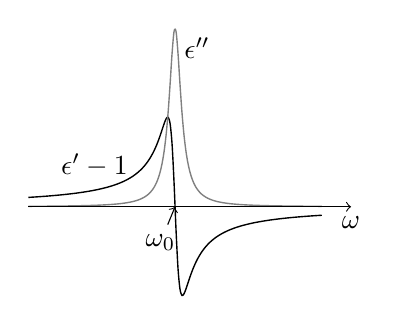
\begin{tikzpicture}[
declare function={ 
 w0 = 100;
 gamma = 1;
 amp = 2;
 epsr(\w) =  amp * (w0 ^2 - \w^2)/ ( (w0 ^2 - \w^2)^2 + gamma^2 * \w^2);
 epsi(\w) =  amp * gamma * \w / ( (w0 ^2 - \w^2)^2 + gamma^2 * \w^2);
  },
]
%\useasboundingbox (0,0) rectangle (5,5);
%\draw (0,0) rectangle (5,5);

\begin{axis}[no markers,
 samples=150, smooth,
     %     ymin=-0.3, ymax=1,
        axis y line=none,
          axis x line=none,
           width= 6.5cm]
           
\addplot [domain=90:110,  line width=0.5pt]    { epsr(x)};
\addplot [domain=90:110,  line width=0.5pt, gray]    { epsi(x)};

\addplot[->] coordinates   {(90,0) (112, 0)};
\node (s) [anchor= north] at (axis cs: 112,0) {$\omega$} ;
\node (w0) [anchor= north ] at (axis cs: 99,-0.002) {$\omega_0$} ;
\draw[->] (w0) -- (axis cs: 100,0);


\node [anchor= north] at (axis cs: 94.5,0.007) {$\epsilon' -1 $} ;
\node [anchor= north] at (axis cs: 101.5,0.02) {$\epsilon'' $} ;

%  
%\addplot[->] coordinates   {(0,0) (6.5, 0)};
%\addplot[] coordinates   {(0,0) (0, -0.03)};
%
%
%\node[anchor=north] at (axis cs: 6.5,0) {$R$};
%\node[anchor=north] at (axis cs: 0,0) {$0$};
%
%\node[anchor=north] at (axis cs: 4,0.3) {$S(R)$};
%\node[anchor=north] at (axis cs: 2,0.25) {$C(R)$};
%\node[anchor=north] at (axis cs: 2,-0.1) {$A(R)$};
%
%
%\node[anchor=north] at (axis cs: +1,0) {$\mathbf{r}_2$};
%
%\node[anchor= north east] at (axis cs: -1,1) {$|\phi_1|^2$};
%\node[anchor= west] at (axis cs: +1.3,-0.7) {$\frac{-1}{|\mathbf{r} - \mathbf{r}_2|}$};
%
%\node (s) [anchor= west] at (axis cs: +1,+0.5) {$\frac{|\phi_1|^2}{|\mathbf{r} - \mathbf{r}_2|}$} ;
%
%\node (k) at (axis cs: -1,+0.) {};

%\draw (s) -- (k) ;

%\node[anchor= south] at (axis cs: 0,0) {$\phi_1 \cdot \phi_2$};

%\node[anchor=west] at (axis cs: 1,1.4) {state $e$};
           
\end{axis}

\end{tikzpicture}


\end{document}